
\setlength{\parskip}{1em}   

\section*{Welcome aboard!}

We look forward to welcoming you to the social evening on Friday at Cap San Diego (7 pm – 2 am)! This iconic ship, docked in Hamburg, provides a unique maritime atmosphere for our event.

The entrance to the social evening begins directly after the conference program at 7 pm. Enjoy an international vegan and vegetarian buffet. Eight complimentary drinks are included in the ticket price.

At 10 pm, we will present the Poster prizes and the award for best supervision. Regrettably, we must inform you that the PuG Band had to cancel their performance this year. Nevertheless, we are confident that the evening will still be an excellent opportunity for exchange and enjoyment, with a live DJ ensuring a vibrant end to the night.

Students and PhD students with a party ticket can enter from 9:30 pm on. Their ticket includes four complimentary drinks.

Join us for an evening of networking, entertainment, and culinary delights at Cap San Diego! 

\textbf{Please be advised that ONLY CASH payments will be accepted on board!}

\vspace*{1cm}

\begin{figure}[H]
	\centering
	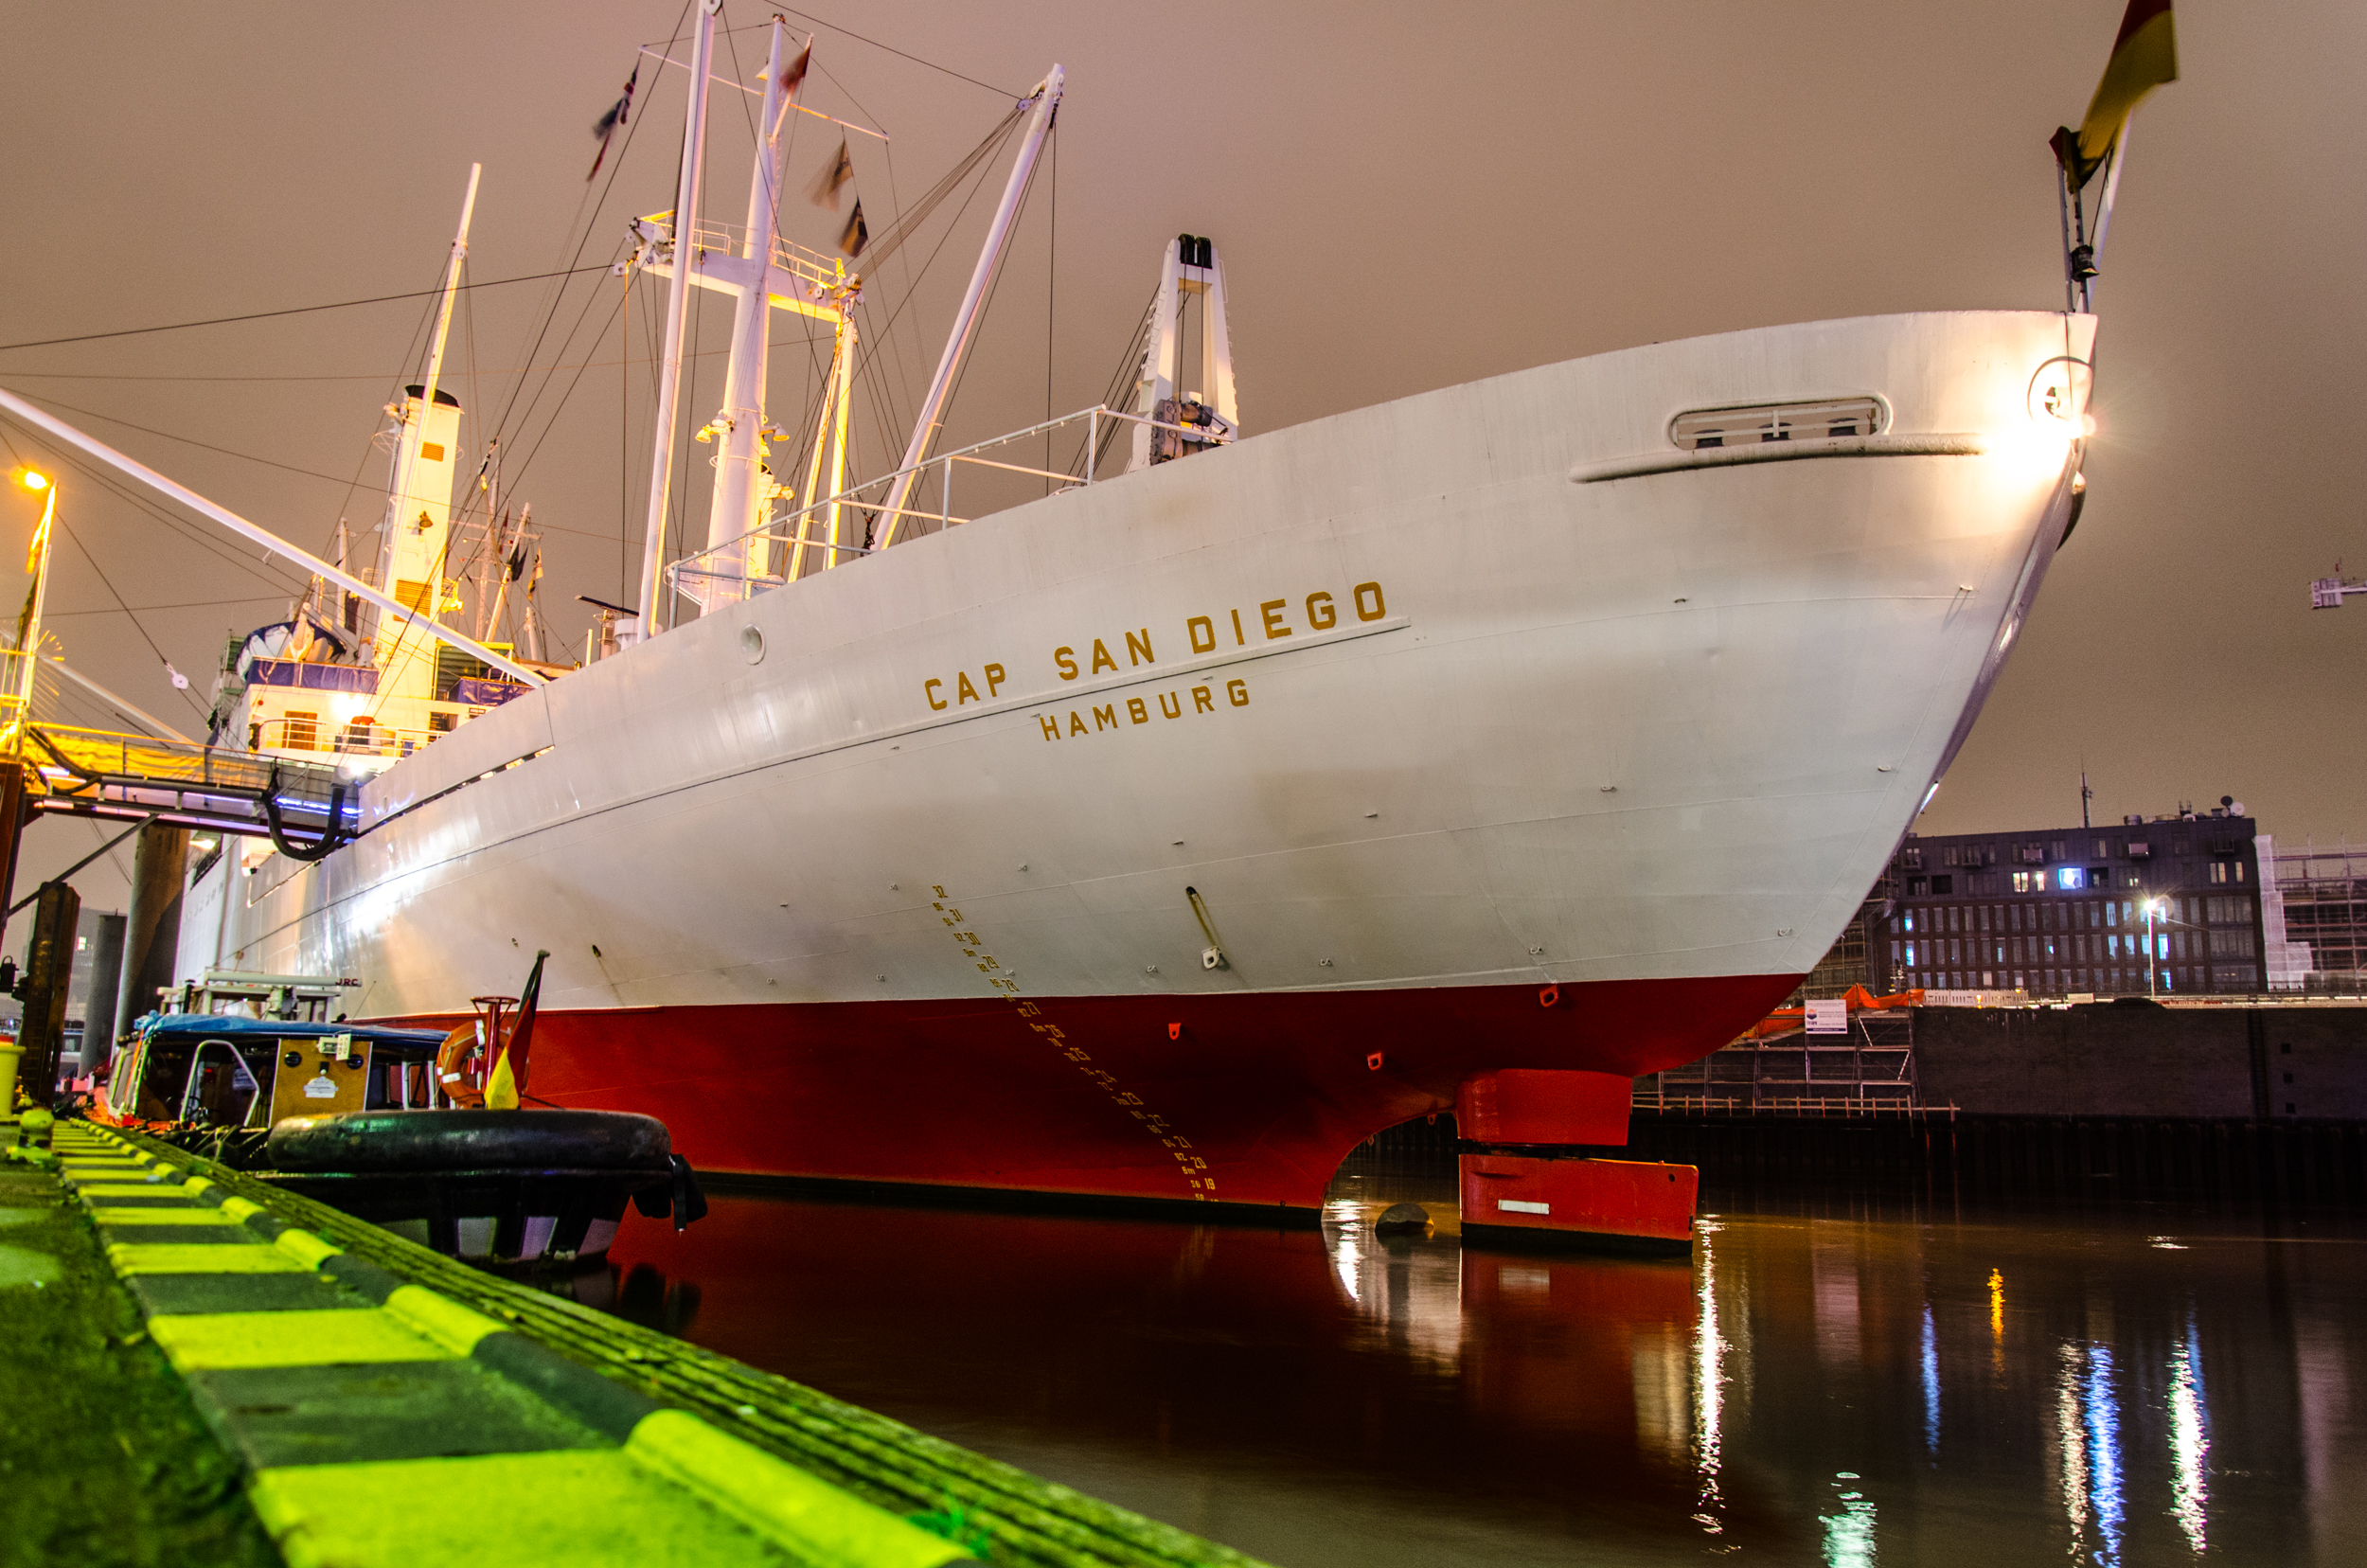
\includegraphics[width=0.7\textwidth]{tex/images/social_event/social4.png}
\end{figure}

\newpage

\section*{How do I get to the social evening?}

\textbf{In a nutshell} \\
The social evening will be held at Cap San Diego, 
which is a museum ship located at Überseebrücke in the Port of Hamburg. 
Please keep in mind that \underline{only cash payment} is possible on the Cap San Diego. 

Date: Friday, 31st May 2024 \\
Adress: Cap San Diego, Überseebrücke, 20459 Hamburg
\begin{figure}[H]
	\centering
	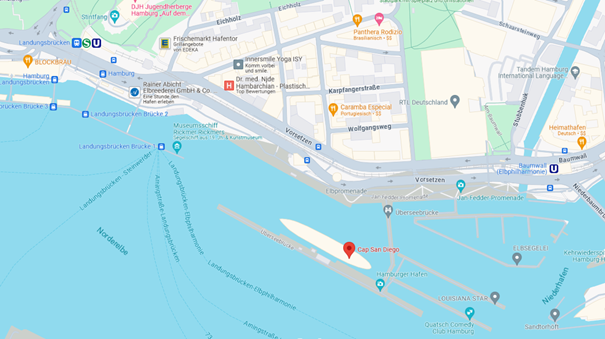
\includegraphics[width=\textwidth]{tex/images/social_event/social_event_karte.png}
\end{figure}

\textbf{By Public Transport:}
\begin{itemize}
	\item S-Bahn: S1 or S3 to Landungsbrücken (5-minute walk).
	\item U-Bahn: U3 to Baumwall (7-minute walk).
	\item Bus: Lines 111 and 112 to Landungsbrücken (5-minute walk).
\end{itemize}

\textbf{By MOIA:}
\begin{itemize}
	\item Book a shared ride via the MOIA app.
\end{itemize}

\textbf{By Stadtrad:}
\begin{itemize}
	\item Hamburg’s bike-sharing service, Stadttrad has stations throughout the city. Pick up a bike from any station and drop it off at Landungsbrücken. The first 30 minutes are free after registration.
\end{itemize}

\newpage

\section*{How do I get home later tonight?}

\vspace*{0.5cm}
\textbf{Night Buses:}
\begin{itemize}
	\item Night Bus Network: Buses with a 600 numbers run all night. Check HVV app for routes 
	\item S-Bahn and U-Bahn: Most lines operate all night on Friday and weekends. Check the HVV app for schedules and routes.
	
\end{itemize}

\vspace*{0.5cm}
\textbf{MOIA:}
\begin{itemize}
	\item Available late at night via the app.
\end{itemize}

\vspace*{0.5cm}
\textbf{Taxi:}
\begin{itemize}
	\item Hansa Taxi: +49 40 211211
	\item Taxi Hamburg: +49 40 666666
	\item Taxiruf: +49 40 441011
	\item Das Taxi Hamburg: +49 40 221122
	
\end{itemize}

\vspace*{0.5cm}
\textbf{Stadtrad:}
\begin{itemize}
	\item Bikes available late at night.
\end{itemize}

\vspace*{1cm}

\begin{center}
	Enjoy your evening and travel safely!
\end{center}

\begin{figure}[H]
	\centering
	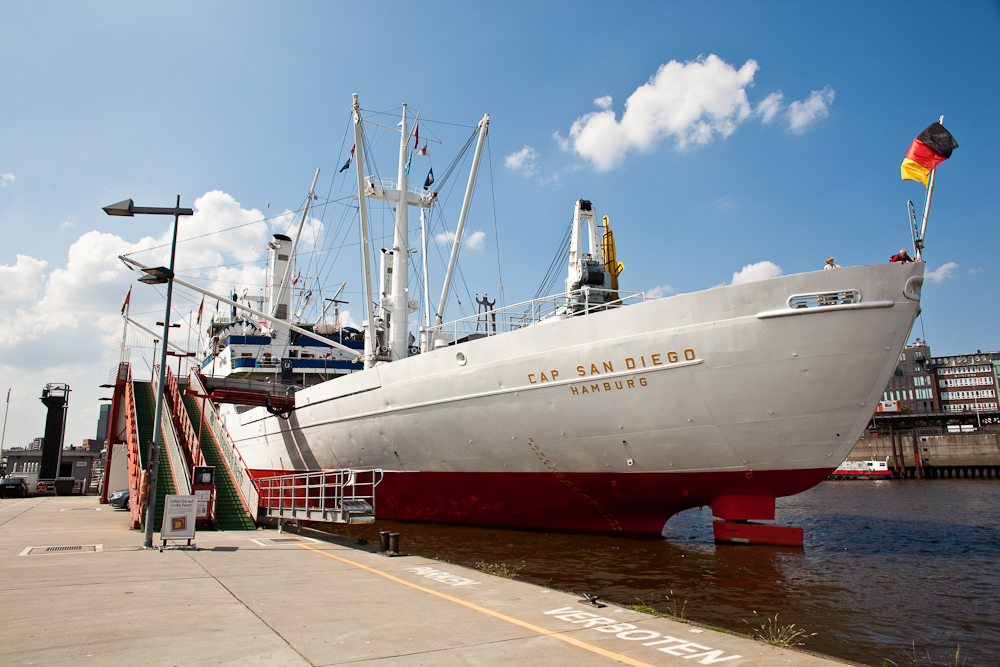
\includegraphics[width=0.3\textwidth, height=3.5cm]{tex/images/social_event/san_diego.jpg}
	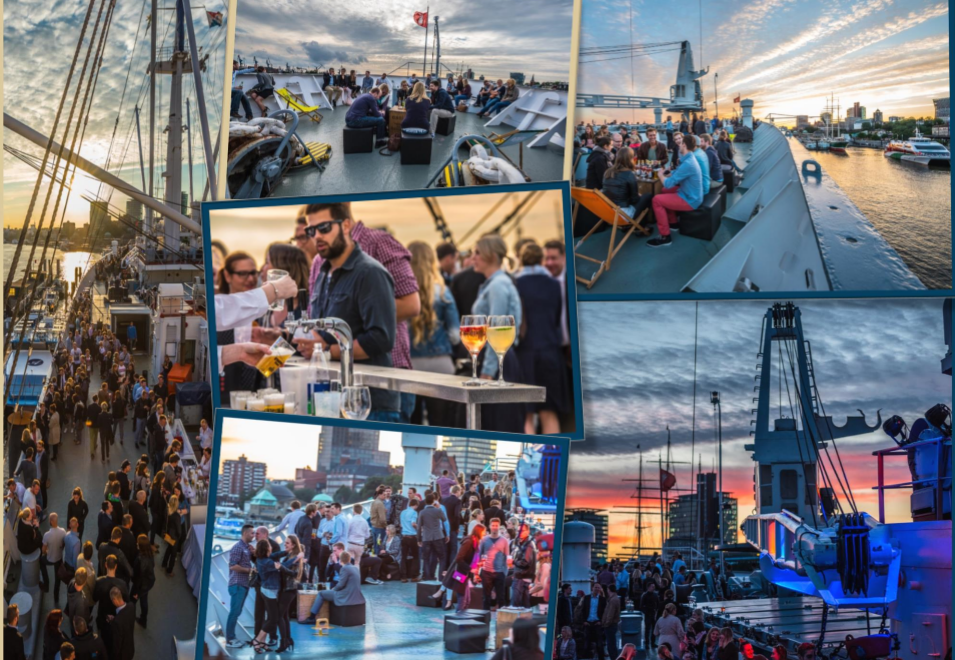
\includegraphics[width=0.3\textwidth, height=3.5cm]{tex/images/social_event/Collage_Open_Air.PNG}
	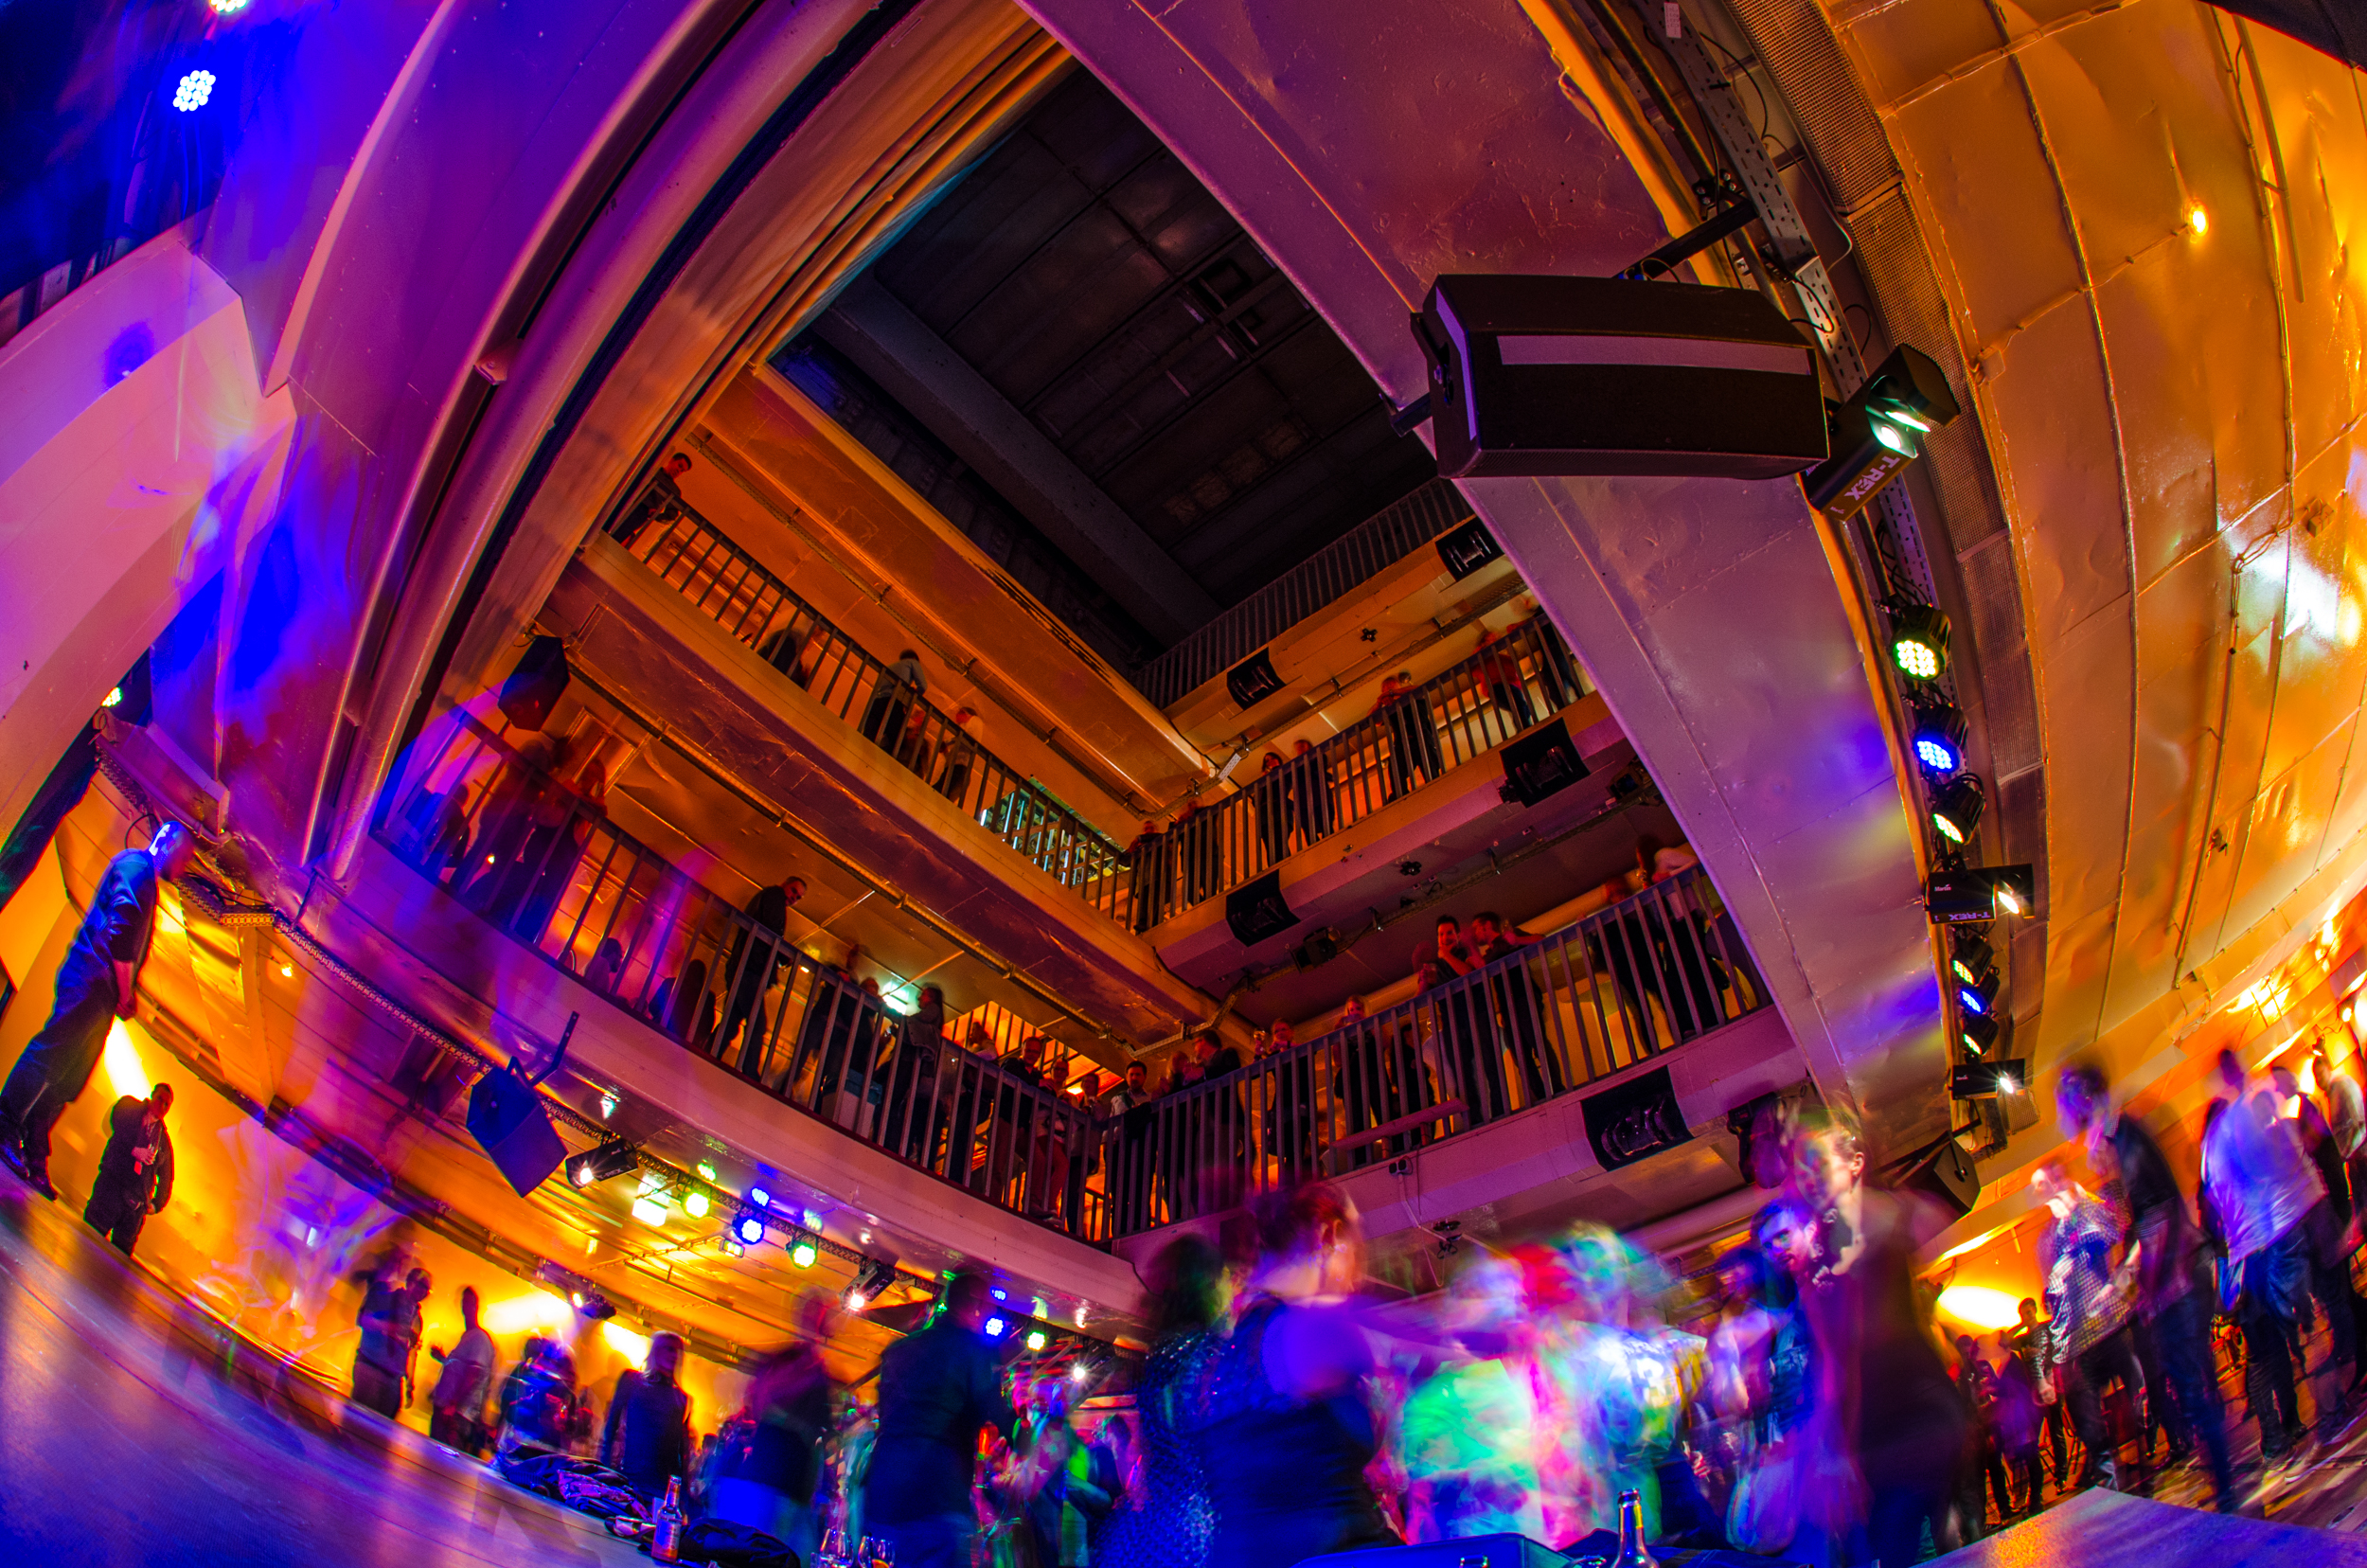
\includegraphics[width=0.3\textwidth, height=3.5cm]{tex/images/social_event/indoor_deck.jpg}
\end{figure}